%==================================%
%-->    Lab: The Op-Amp         <--%
%--> Author: Charles Edward Pax <--%
%-->   Date: 2006.02.28         <--%
%==================================%
%
\documentclass[11pt,onecolumn]{article}

\usepackage{color,graphics}

\begin{document}
\title{The Op-Amp}
\date{\today}
\author{Charles Edward Pax}
\maketitle

%=====================%
%--> Sec: Abstract <--%
%=====================%
\abstract{Simple inverting and noninnverting amplifier circuits are examined and analyzed.}

%=========================%
%--> Sec: Introduction <--%
%=========================%
\section{Introduction}\label{sec:Introduction}
The delicate 741 op-amp is an integrated circuit (IC), which contains 24 transistors, 12 resistors, and 1 capacitor. This IC was hooked up in circuits as shown in Figure \ref{fig:inverting_data} and Figure \ref{fig:noninverting_data} to create an inverting and noninverting amplifier. The offset is adjusted with a 10 k$\Omega$ potentiometer (pot). The power given to the amplifier is $\pm$12 V.
%
% Inverting op-amp
%
\begin{figure}
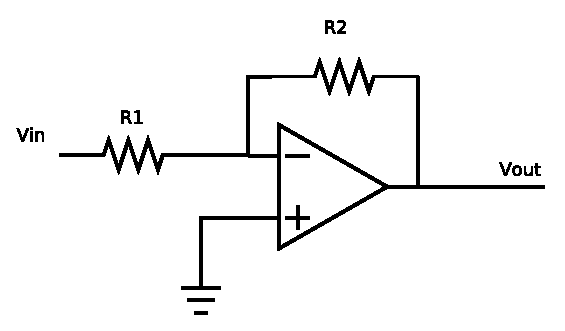
\includegraphics{Diagram1.eps}
\caption{Inverting op-amp.}\label{fig:inverting_data}
\end{figure}
%
% Noninverting op-amp
%
\begin{figure}
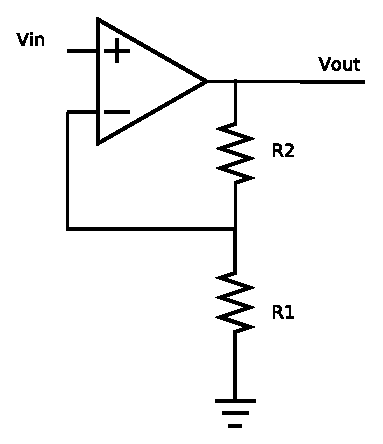
\includegraphics{Diagram2.eps}
\caption{Noninverting op-amp.}\label{fig:noninverting_data}
\end{figure}


%=================%
%--> Sec: Data <--%
%=================%
\section{Data}\label{sec:Data}
For the circuits in Figure \ref{fig:inverting_data} and Figure \ref{fig:noninverting_data}, $R_1$ was set to 1 K$\Omega$ and $R_2$ was varried in order to set the magnitude of the gain to be approximatly 1, 10, and 100, while insuring the input voltage is small enough such that the output would be less than 10 V. These measured values are listed in Table \ref{tab:Q1_inverting} and Table \ref{tab:Q1_noninverting} for the inverting and noninverting circuits respectivly.
\begin{table}
\center
\begin{tabular}{|lllll|}
\hline
$R_2$ (k$\Omega$)& $V_{in}$ (V)	& $V_{out}$ (V)	& Gain	& Offset \\
\hline
0		& -0.11		& -0.11		& 1	& 0 \\
0.1		& -0.11		& -0.13		& 1.182	& \\
0.39		& -0.11		& -0.16		& 1.455	& \\
0.51		& -0.11		& -0.18		& 1.64	& \\
2.7		& -0.11		& -0.44		& 4	& \\
5.1		& -0.11		& -0.71		& 6.46	& \\
7.5		& -0.10		& -0.95		& 8.64	& \\
10		& -0.10		& -1.16		& 10.55	& -1.04 \\
100		& -0.05		& -5.44		& 108.0	& -5.32 \\
\hline
\end{tabular}
\caption{Values for the inverting circuit.}\label{tab:Q1_inverting}
\end{table}

\begin{table}
\center
\begin{tabular}{|llll|}
\hline
$R_2$ (k$\Omega$)& $V_{in}$ (mV)& $V_{out}$ (mV)& Gain	\\
\hline
0.01		& 3.3		& 3.1		& 0.939 \\
1		& 3.3		& 6.2		& 1.878 \\
10		& 3.3		& 31.4		& 10.33 \\
20		& 3.3		& 65.4		& 20.43 \\
100		& 3.3		& 319		& 106.3 \\
\hline
\end{tabular}
\caption{Values for the noninverting circuit.}\label{tab:Q1_noninverting}
\end{table}

$V_{in}$ was connected to ground to check if there is an offset voltage in the output. The offsets are listed in Table \ref{tab:Q2}.

\begin{table}
\center
\begin{tabular}{|ll|}
\hline
$R_2$ (k$\Omega$)	& $V_{off}$ (V) \\
\hline
1			& 0.006 \\
5.1			& 0.02 \\
10			& 0.03 \\
20			& 0.07 \\
51			& 0.172 \\
100			& 0.337 \\
270			& 0.792 \\
\hline
\end{tabular}
\caption{Offset voltages.}\label{tab:Q2}
\end{table}

$V_{out} / V_{in}$ was measured using the digital multimeter (DMV) for several in DC voltage levels. To obtain the desired low voltage for the input, a voltage divider was constructed. The inverting op-amp saturated at -9.7 V with an input of  0.1 V, while the noninverting op-amp input voltage saturated to a maximun at 11.30 V with an input of 0.111 V. The input voltage and the current $I_1$ through $R_1$ and the input impedance for one gain setting of the of the inverting amplifier were measured\footnote{Answer this question.}.

The function generator was employed to input a sine wave to the inverting op-amp. The gain and phase shift were measured and recorded in Table \ref{tab:Q3} for a circuit setup with a gain of 100. The phase shift and gain are plotted against frequency in Figure \ref{fig:phase} and Figure \ref{fig:freq} respectivly. It can be observed that the amplifier gain decreases at high frequencies.
\begin{table}
\center
\begin{tabular}{|lllll|}
\hline
$f$ (kHz)& Gain	& Phase	& $V_{in}$ (V)	& $V_{out}$ (V) \\
\hline
1.588	& 0.212	& 0	& 0.85		& 0.18 \\
3.12	& 0.200	& 80	& 0.85		& 0.17 \\
6.97	& 0.182	& 60	& 0.85		& 0.155 \\
11.04	& 0.159	& 40	& 0.85		& 0.135 \\
16.27	& 0.141	& 30	& 0.85		& 0.12 \\
21.66	& 0.129	& 25	& 0.85		& 0.11 \\
30.8	& 0.112	& 19	& 0.85		& 0.095 \\
41.0	& 0.941	& 16	& 0.85		& 0.08 \\
\hline
\end{tabular}
\caption{Measurements for the sine wave input.}\label{tab:Q3}
\end{table}
%
% Inverting phase graph
%
\begin{figure}
\center
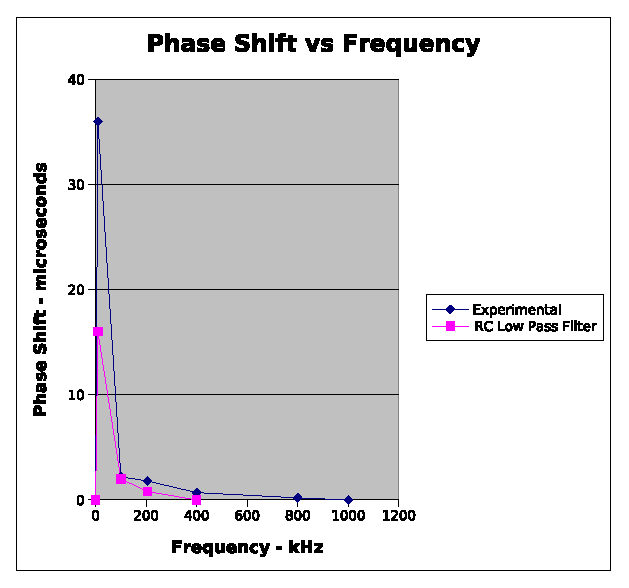
\includegraphics{phase.eps}
\caption{Phase shift versus frequency in an inverting amplifier circuit.}\label{fig:phase}
\end{figure}
%
% Inverting gain graph
%
\begin{figure}
\center
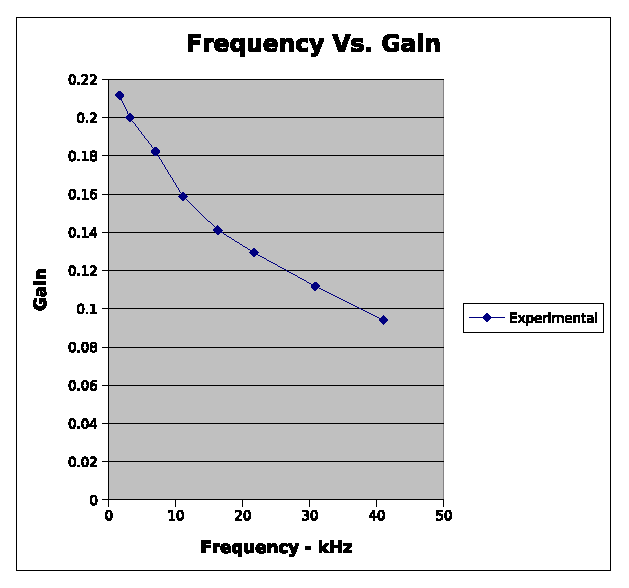
\includegraphics{freq.eps}
\caption{Gain versus frequency in an inverting amplifier circuit.}\label{fig:freq}
\end{figure}

Figure \ref{fig:freq} shows how the measured decrease in gain from the inverting op-amp compare to a RC low pass fileter. We can see\footnote{Answer this question.}. The equivalent corner frequency is\footnote{Answer this question.}.

At 50 and 500 kHz, for a gain of 100 in the inverting amplifier, the input amplitude was increased and the change in the output waveform was observed.
\begin{figure}
\center
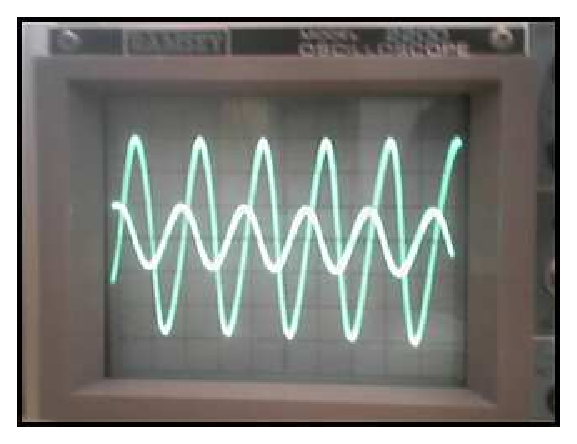
\includegraphics{sketch.eps}
\caption{Change in waveform.}\label{fig:sketch}
\end{figure}

%=======================%
%--> Sec: Discussion <--%
%=======================%
\section{Discussion \& Analysis}\label{sec:Discussion_and_Analysis}
The limitations of the op-amp include the finite gain and the finite $V_{out}$ due to saturation. With a AC input there is a finite bandwidth and in DC there is a finite input resistance.


%=========================%
%--> Sec: Bibliography <--%
%=========================%
%\begin{thebibliography}{9}
% This command tells LaTeX to create "References" section containing all the references that are not commented out. Be sure to uncomment all the references which you use and add those that are not currently listed.
%\bibitem{Manual} Lab manual
%\end{thebibliography}

\end{document}

%=================%
%--> Templates <--%
%=================%
% This section contains templates for commonly used environments. This section will not appear in you final document as it come after the "\end{document}" command above.

% Equation template
\begin{equation}\label{eq:eqLabel}
math = good^2
\end{equation}

% Figure template
\begin{figure}
\input{graphicFile}
\caption{This is the caption. It should include a short description of the figure.}\label{fig:figureLabel}
\end{figure}

% Table template
\begin{table}
\center
\begin{tabular}{|lll|}
\hline
Number	& Number$^2$ \\
1	& 1 \\
2	& 4 \\
3	& 9 \\
\hline
\caption{This is a caption.}\label{tab:squaring}
\end{table}
